\cleardoublepage

\chapter{Wprowadzenie do przetwarzania języka naturalnego}
W tym rozdziale przedstawiono podstawowe definicje i pojęcia kryjące się za terminem \enquote{przetwarzanie języka naturalnego} (ang. \textit{natural language processing — NLP}). Zaprezentowano także ewolucję chatbotów i różne podejścia do rozwoju NLP ze szczególnym uwzględnieniem metod uczenia maszynowego.


    \section{Definicja przetwarzania języka naturalnego}
    Określenie \enquote{język naturalny} stosuje się, aby odseparować język ludzki (np. polski, włoski czy chiński) od języka formalnego (np. Python, C++ czy XML). Język naturalny był rozwijany przez ludzi na drodze długofalowej ewolucji. Służy do komunikacji oraz wyrażania myśli i emocji w formie werbalnej. Język formalny zaś, składający się z symboli przystępnych do zrozumienia dla człowieka, zapewnia doskonałą komunikację między programistą a maszyną. Dzięki swojej precyzji umożliwia tworzenie m.in. zaawansowanych aplikacji komputerowych oraz skryptów.
    
    Przetwarzanie języka naturalnego  to technika pozwalająca komputerom interpretować i generować ludzki język. NLP umożliwia maszynom analizę ludzkich słów i reagowanie na nie w sposób sensowny i naturalny. Tą interdyscyplinarną technikę tworzą trzy główne dziedziny: sztuczna inteligencja, informatyka oraz lingwistyka. Przedstawiono to na diagramie \ref{nlp_diagram}.

    \begin{center}
        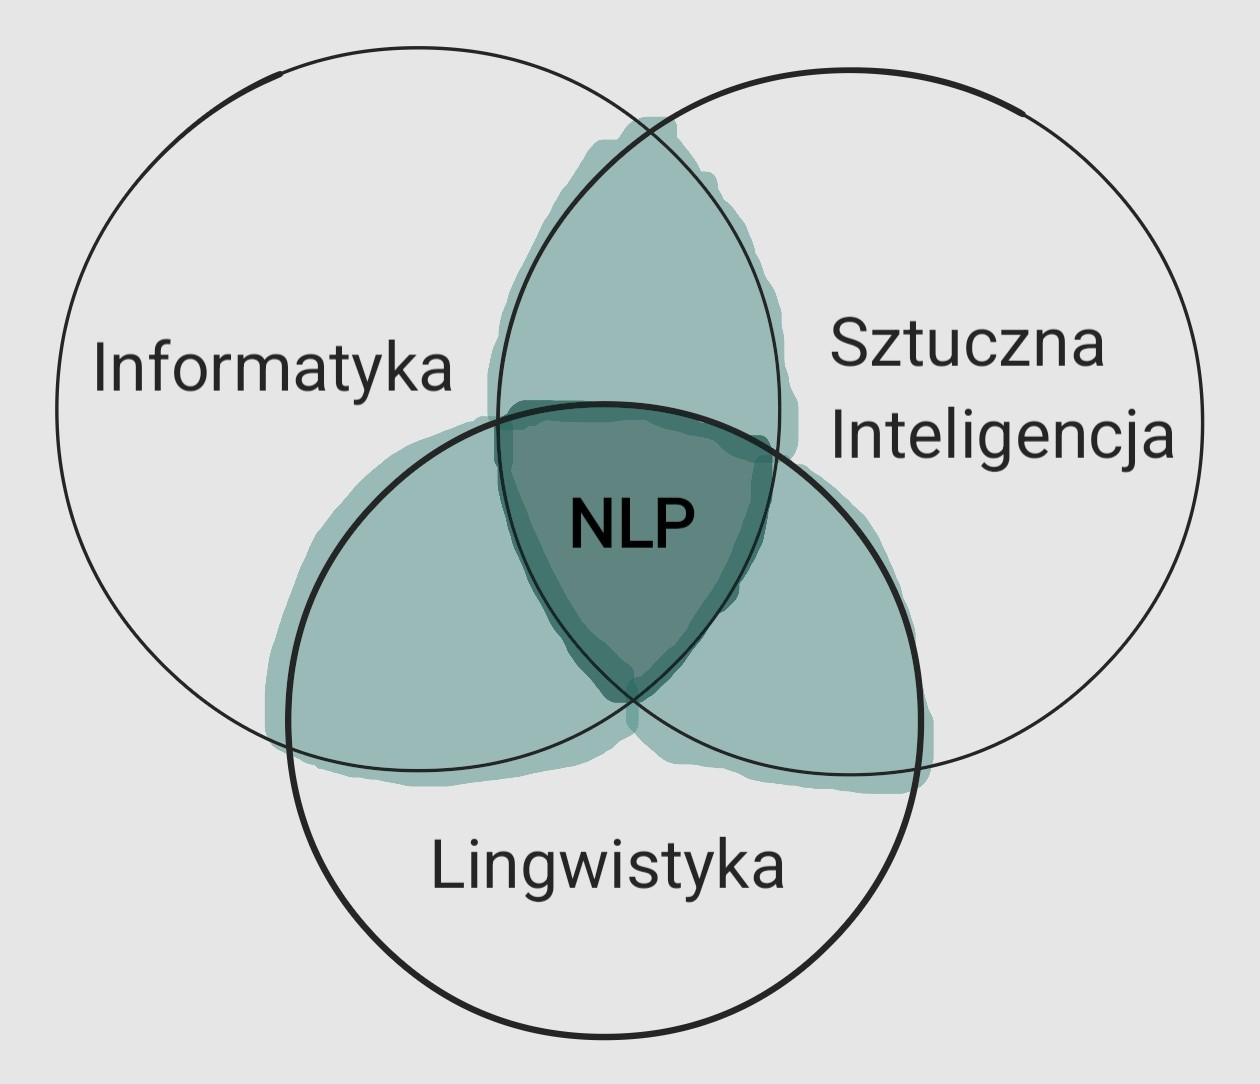
\includegraphics[width=0.5\textwidth]{rysunki/nlp_diagram.jpg}
        \captionof{figure}{ Diagram przedstawiający trzy dziedziny, które współtworzą przetwarzanie języka naturalnego \cite{krohn2022uczenie} }
        \label{nlp_diagram}
    \end{center}

    Przetwarzanie języka naturalnego stosuje się zarówno w kontekście języka pisanego, jak i mówionego. Technologie i algorytmy z tej dziedziny mają swoje zastosowania w następujących obszarach:
    \begin{itemize}
        \item tłumaczenie z jednego języka na inny,
        \item analiza sentymentu,
        \item wyszukiwarki kontekstowe,
        \item prowadzenie konwersacji z komputerem (chatboty).
    \end{itemize}


    \section{Definicja chatbota}
    Chatbotem nazywa się oprogramowanie wykorzystujące NLP, które za pomocą interfejsu graficznego lub głosowego umożliwia człowiekowi konwersację z komputerem, do złudzenia przypominającą rozmowę dwóch użytkowników. Chociaż początki tego rozwiązania sięgają już połowy dwudziestego wieku, to dopiero w ostatnich latach stały się one bardzo popularne i przełomowe w obszarze sztucznej inteligencji za sprawą wykorzystania dużych modeli językowych.
    
    
    \section{Zarys historyczny chatbotów}
    Znaczący wkład w rozwój przetwarzania języka naturalnego, w tym chatbotów, wniósł w 1950 roku brytyjski matematyk i informatyk Alan Turing. W artykule \enquote{Computing Machinery and Intelligence} pionier szukał odpowiedzi na pytanie \enquote{Czy maszyny potrafią myśleć?} \cite{turing1950}. W ramach tego zagadnienia, stworzył test, który nazwano testem Turinga. Polegał on na tym, że osoba badana, inaczej zwana sędzią, prowadziła dwie konwersacje: jedną z drugim człowiekiem, a drugą z komputerem. Jeżeli badany nie był w stanie jednoznacznie rozróżnić, który dialog był prowadzony z chatbotem, komputer pozytywnie przechodził test.

    
        \subsection{ELIZA}
        W 1966 roku niemiecki informatyk Joseph Weizenbaum, zainspirowany testem Turinga, napisał w języku SLIP program symulujący konwersację z psychoanalitykiem. Chatbot został nazwany ELIZA na cześć głównej bohaterki dramatu Pigmalion, Elizy Doolittle. Program używał prostych technik rozpoznawanie słów kluczowych, dopasowania wzorców (ang. \textit{pattern matching}) i mechanizmu substytucji. Poniżej przedstawiono przykładowy dialog, prezentujący jak ELIZA przekształcała zdania użytkownika w swoich odpowiedziach \cite{from_eliza_to_chatgpt2024}:

        \begin{enumerate}
            \item You: Well, my boyfriend made me come here.\newline
                ELIZA: Is it important to you that your boyfriend made you come here ?
            \item You: He says I'm depressed much of the time.\newline
                ELIZA: I am sorry to hear that you are depressed.
            \item You: It is true. I'm unhappy.\newline
                ELIZA: Can you explain what made you unhappy ?
        \end{enumerate}

        Trudności w odróżnieniu chatbota od drugiego człowieka spowodowały, że niektórzy użytkownicy za bardzo przywiązywali się do programu, wierząc, że ich rozumie. Rezultatem tego, było zdefiniowanie zjawiska psychologicznego, które nazwano efektem Elizy. Polega ono na tym, że człowiek przypisuje maszynie ludzkie cechy, takie jak empatię, zrozumienie czy inteligencję.


        \subsection{PARRY}
        W 1972 roku amerykański psychiatra Kenneth Colby napisał w języku MLISP program PARRY. Konwersacja z tym chatbotem miała imitować prowadzenie dialogu z osobą chorą na schizofrenię paranoidalną. Jego zadaniem były prowokacja i wprowadzanie kontrowersji, które miały skłonić użytkownika do pisania dłuższych wypowiedzi \cite{history_of_chatbots2019}. Odpowiedzi programu bazowały na zbiorze zasad zdefiniowanych w logice systemu i były one generowane za pomocą techniki “elaboration” \cite{from_eliza_to_chatgpt2024}. PARRY był znacznie bardziej zaawansowanym rozwiązaniem niż ELIZA.


        \subsection{A.L.I.C.E.}
        Program Artificial Linguistic Internet Computer Entity (ALICE) został napisany w 1995 w języku Java przez amerykańskiego informatyka Richarda Wallace'a. Baza wiedzy systemu przechowywana była w plikach AIML, stanowiących implementację standardu XML. W latach 1995-2000 społeczność Alicebot zapewniła funkcjonalność, umożliwiającą użytkownikom dodawanie wzorców konwersacyjnych do bazy wiedzy chatbota \cite{alice2015}. Inteligencja ALICE opierała się na zaawansowanym dopasowywaniu wzorców.


        \subsection{SmarterChild}
        W 2001 roku firma ActiveBuddy udostępniła do powszechnego użytku chatbota SmarterChild. Użytkownicy mogli prowadzić dialog z cyfrowym asystentem za pomocą platform: AOL Instant Messenger, Windows Live Messenger oraz Yahoo Messenger. Nie tylko odpowiadał on na pytania dotyczące pogody, sportu czy najnowszych wiadomości, ale także grał w gry. System był w stanie uczyć się i ewoluować wraz z każdą interakcją z człowiekiem. Pozwalało mu to na dostosowywanie stylu odpowiedzi znając styl pisania i preferencje użytkownika \cite{from_eliza_to_chatgpt2024}.
    

        \subsection{Siri}
        W 2011 roku firma Apple zaprezentowała Siri, przełomowego asystenta AI, który do dziś jest powszechnie używany w produktach koncernu. Komponując ze sobą przetwarzanie języka naturalnego i uczenie maszynowe, Siri jest w stanie przeanalizować zapytanie użytkownika i zapewnić odpowiednią, spersonalizowaną odpowiedź. Wirtualny asystent pomaga w wykonywaniu najróżniejszych zadań w smartfonie, takich jak wysłanie wiadomości, zestawienie połączeń czy ustawienie budzika \cite{from_eliza_to_chatgpt2024}.

        
    \section{Podejścia do przetwarzania języka naturalnego}
    Metody rozwiązywania problemów NLP można podzielić na trzy rodzaje: heurystykę, uczenie maszynowe oraz uczenie głębokie. W tym podrozdziale zwięźle przedstawiono każde z tych podejść.

        \subsection{Metody heurystyczne}
        We wczesnych systemach przetwarzania języka naturalnego oprócz słowników i tezaurusów rozwijano także bardziej złożone bazy wiedzy wspomagające NLP oparte na regułach. Doskonale obrazuje to WordNet \cite{wordnet_d3}. Jest to baza słów i semantycznych relacji między nimi. Do takich relacji zalicza się:

        \begin{itemize}
            \item synonimy — wyrażenia o takim samym lub zbliżonym znaczeniu, które brzmią i zapisuje się inaczej,
            \item hiponimy — słowa o znaczeniu węższym, które nazywają konkretny rodzaj lub gatunek obiektu z szerszej grupy, np. \enquote{arabski} i \enquote{chiński} to hiponimy języka obcego,
            \item meronimy — słowa nazywające część składową, która współtworzy większą całość, np. \enquote{silnik} i \enquote{kierownica} to meronimy samochodu.
        \end{itemize}

        \noindent Na rysunku \ref{heurystyka_transport_publiczny} przedstawiono wizualizację takich relacji między słowami w bazie WordNet.

        \begin{center}
            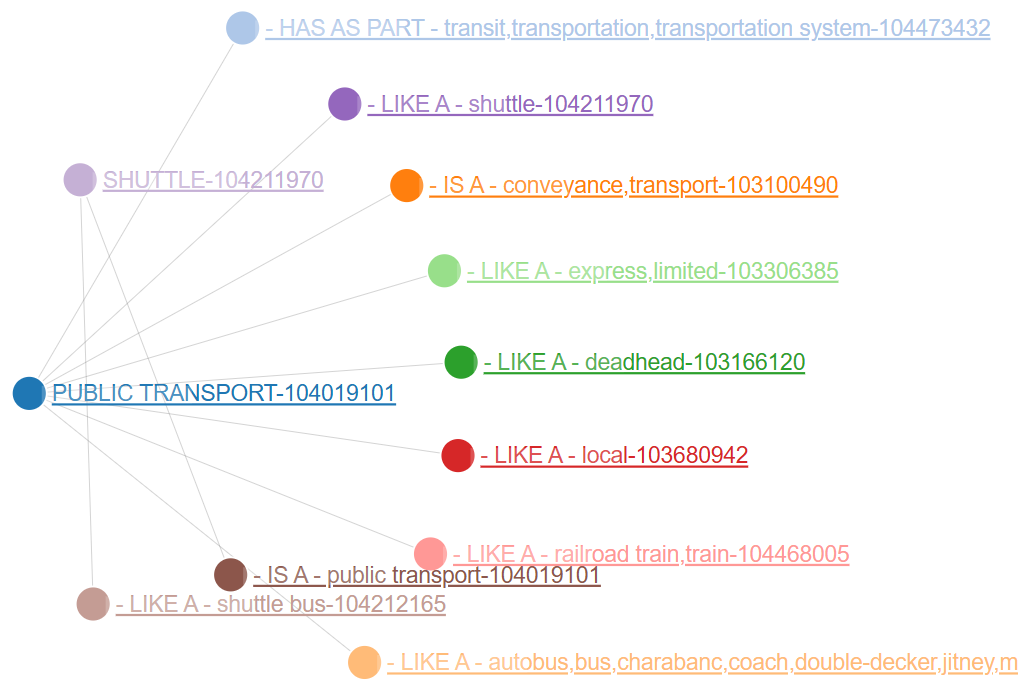
\includegraphics[width=0.6\textwidth]{rysunki/heurystyka_transport_publiczny.png}
            \captionof{figure}{ Graf bazowy WordNet w języku angielskim dla wyrażenia \enquote{public transport} \cite{wordnet_d3} }
            \label{heurystyka_transport_publiczny}
        \end{center}
        
        Ponadto, doskonałym sposobem na analizowanie tekstu są wyrażenia regularne, inaczej zwane regeksami (ang. \textit{regex}). Regeks jest sekwencją znaków, która definiuje wzorzec stosowany do dopasowania i szukania słów w tekście. Wyrażenia regularne stosowane są po to, aby dodawać do systemu wiedzę z konkretnego zakresu. Dobrym przykładem użycia wyrażeń regularnych będzie program, który na podstawie numeru kierunkowego określa, czy dzwoniący klient pochodzi z Polski czy z zagranicy, aby w razie potrzeby zestawić połączenie z konsultantem mówiącym w języku angielskim. Regeksy można podzielić na: 
        
        \begin{itemize}
            \item probabilistyczne — określają prawdopodobieństwo dopasowania szukanego słowa do wzorca,
            \item deterministyczne — określają zero-jedynkowo czy szukane słowo pasuje do wzorca.
        \end{itemize}

        Innym przydatnym narzędziem, używanym do modelowania języka naturalnego, jest gramatyka bezkontekstowa (ang. \textit{context-free grammar} — CFG). Wykorzystuje się ją do znacznie głębszej analizy niż wyżej opisany regeks. Jak trafnie opisano w książce \cite{sowmya_ksiazka_nlp2023}, \enquote{CFG można wykorzystać do wyodrębniania bardziej skomplikowanych, hierarchicznych informacji, które mogłyby umknąć wyrażeniu regularnemu}. Formalnie CFG definiowana jest jako czwórka $G=(N,T,P,S)$, gdzie $N$ jest zbiorem nieterminali, $T$ jest alfabetem terminalnym, $P$ jest zbiorem reguł w postaci $A \rightarrow \alpha$, a $S$ stanowi symbol początkowy gramatyki. Język generowany przez $G$, oznaczany jako $L(G)$, jest zbiorem słów nad alfabetem $T$ osiągalnych z symbolu startowego $S$ i stosujących reguły gramatyki $P$.


        \subsection{Metody reprezentacji tekstu}
        W nowoczesnych systemach przetwarzania języka naturalnego, oprogramowanie dokonuje segmentacji tekstu na zdania i słowa. Tak wydzielone struktury danych definiuje się jako tokeny. W zależności od rodzaju segmentacji, technikę tę nazywa się tokenizacją zdaniową lub wyrazową. Jak trafnie podają autorzy książki \cite{zaawansowane_techniki_NLP2025}, \enquote{proces tokenizacji jest ważnym wstępnym etapem w wielu zadaniach NLP, ponieważ przekształca on nieustrukturyzowane dane tekstowe w ustrukturyzowany format, który można analizować z użyciem algorytmów uczenia maszynowego lub innych technik}. Na poniższym rysunku \ref{nltk_tokenizer} zaprezentowano przykład tokenizacji wyrazowej z wykorzystaniem biblioteki Natural Language Tool Kit (NLTK).

        \begin{center}
            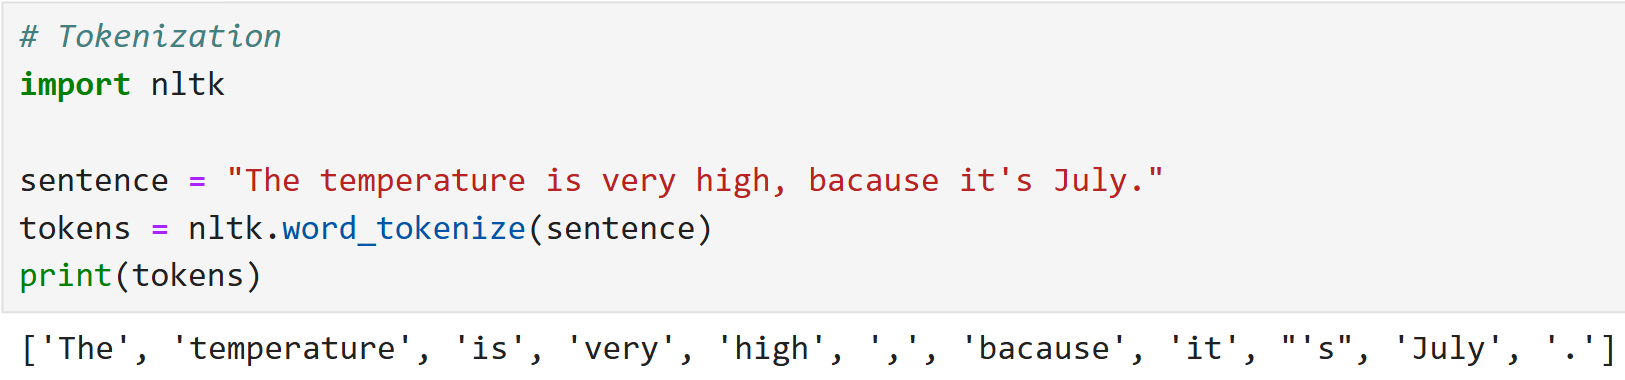
\includegraphics[width=0.8\textwidth]{rysunki/nltk_tokenizer.png}
            \captionof{figure}{ Przykład tokenizacji wyrazowej wykonanej przy użyciu biblioteki NLTK \cite{nltk_tokenization_library}}
            \label{nltk_tokenizer}
        \end{center}

        \noindent Kolejnymi ważnymi zagadnieniami w kontekście wstępnego przetwarzania tekstu są lematyzacja (ang. \textit{lemmatization}) oraz tematyzacja (ang. \textit{stemming}). Pierwszy termin odnosi się do uproszczenia słowa do jego postaci podstawowej lub słownikowej, nazywanej lematem. Pozwala to na traktowanie słowa jako znormalizowany wyraz. Drugi termin dotyczy redukcji słów do formy pozbawionej końcówek, nazywanej tematem. Celem tego zabiegu jest ujednolicenie różnych odmian i wariantów wyrazu poprzez przypisanie ich do wspólnej formy podstawowej. Na rysunku \ref{nltk_lem_stem} przedstawiono przykłady obydwu tych zagadnień z wykorzystaniem biblioteki NLTK.

       \begin{center}
            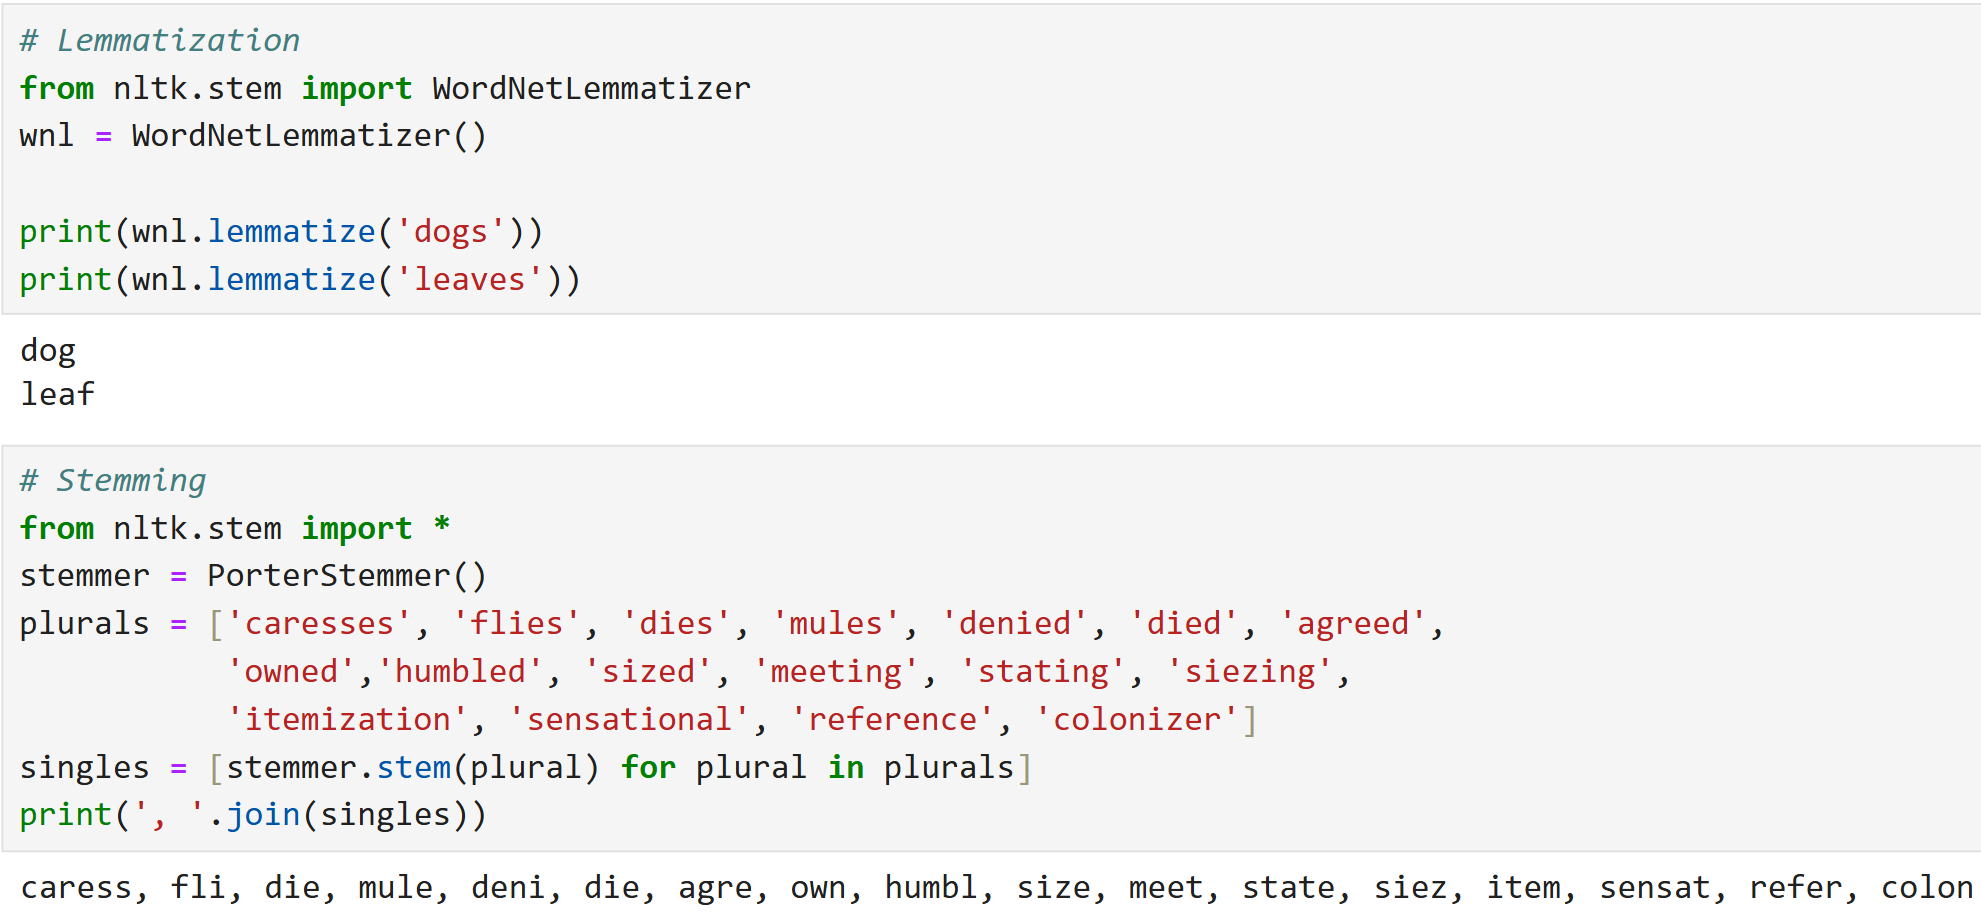
\includegraphics[width=0.85\textwidth]{rysunki/nltk_lem_stem.png}
            \captionof{figure}{ Przykład lematyzacji i tematyzacji wykonanych przy użyciu biblioteki NLTK \cite{nltk_tokenization_library}}
            \label{nltk_lem_stem}
        \end{center}

        Po wstępnym przygotowaniu tekstu następuje proces reprezentacji, który jest szczególnie ważny w kontekście uczenia maszynowego. Do klasycznych i najbardziej popularnych metod zalicza się: 

        \begin{itemize}
            \item worek słów (ang. \textit{bag of words} — BoW) — prosta i powszechnie stosowana metoda konwersji ciągu wyrazów na wektor liczb, które określają częstotliwości występowania przetwarzanych słów, zważając na kolejność ich występowania i kontekst,
            \item worek n-gramów — uogólniona funkcjonalność BoW uwzględniająca kolejność występujących słów w sekwencji,
            \item TF-IDF — technika ilustrująca ważność słów w bloku tekstowym, uwzględniająca nie tylko częstotliwość, lecz także rzadkość ich występowania,
            \item word2vec — technika posiadająca architekturę CBOW lub skip-gram, umożliwiająca tworzenie wielowymiarowych wektorowych reprezentacji słów, inaczej zwanych osadzeniami (ang. \textit{embeddings}) oddającymi znaczenia wyrażeń i ich wzajemne relacje.
        \end{itemize}

        
        \subsection{Uczenie maszynowe w NLP}
        Uczenie maszynowe (ang. \textit{machine learning} — ML) jest poddziedziną sztucznej inteligencji, którą współtworzą trzy główne dziedziny: informatyka, robotyka i statystyka. Są to odpowiednio zaprogramowane algorytmy potrafiące się doskonalić (uczyć) z danych bez ingerencji programisty. Jak trafnie opisano w lekturze \cite{sowmya_ksiazka_nlp2023} \enquote{każde podejście do NLP oparte na uczeniu maszynowym, nadzorowanym czy nie, zwykle składa się z trzech etapów: ekstrakcja cech z tekstu, użycie reprezentacji cech do uczenia modelu oraz ocenianie i ulepszanie modelu}.
        
        Pierwszym wartym uwagi algorytmem jest naiwny klasyfikator bayesowski (ang. \textit{naive bayes classifier}). To bardzo szybkie i łatwe w użyciu podejście jest powszechnie stosowane do wstępnego klasyfikowania tekstów. 
        Na przykład, przy filtrowaniu wiadomości e-maili, jeżeli algorytm wykrył w temacie słowo \enquote{wygrana}, którego występowanie w 90\% przypadków wskazuje na spam, to wiadomość zostanie zaklasyfikowana do tej kategorii. Jak wskazuje nazwa algorytmu, opiera się on na twierdzeniu Bayesa. Twierdzenie to opisano wzorem \ref{wzór_bayesa}, który określa prawdopodobieństwo wystąpienia klasy decyzyjnej $y$, pod warunkiem wystąpienia wektora atrybutów $x$. 

        \begin{equation}
        \begin{aligned}
            P(Y = y | X = x) = \frac{P(X = x | Y = y) P(Y = y)}{P(X = x)}
        \end{aligned}
        \label{wzór_bayesa}
        \end{equation}
        
        Drugim klasycznym podejściem w NLP jest maszyna wektorów nośnych (ang. \textit{support vector machine — SVM}). Algorytm ten może nauczyć się liniowej lub nieliniowej granicy decyzyjnej w celu oddzielenia danych (np. tekstów) należących do różnych klas, zachowując maksymalną odległość między nimi. Pomimo długiego czasu treningu, za sprawą dużej odporności na szumy i zmienność w danych, SVM jest jednym z najskuteczniejszych algorytmów. Na poniższej ilustracji \ref{svm} przedstawiono przykład użycia SVM.

        \begin{center}
            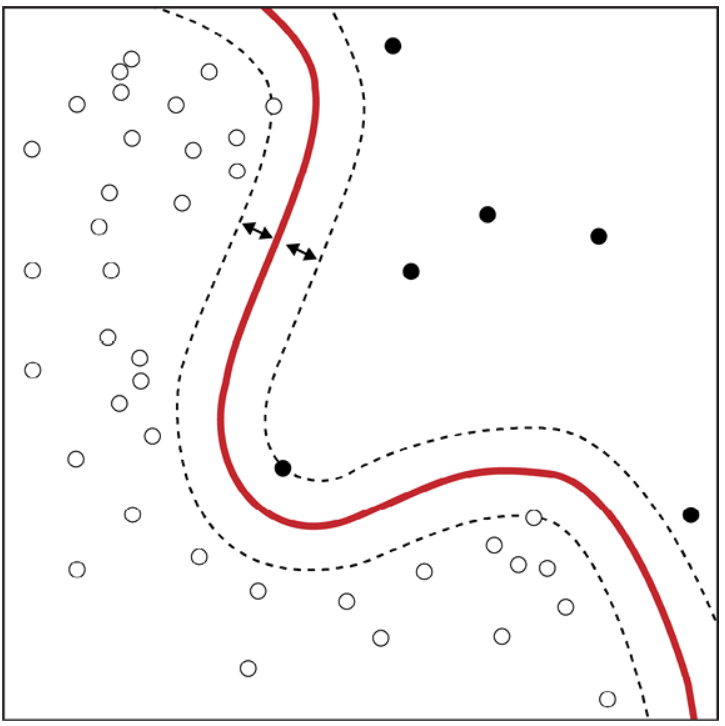
\includegraphics[width=0.4\textwidth]{rysunki/svm.png}
            \captionof{figure}{ Przykład zastosowania SVM dla dwuwymiarowej przestrzeni cech \cite{sowmya_ksiazka_nlp2023}}
            \label{svm}
        \end{center}
        
        
        \subsection{Uczenie głębokie w NLP}
        W ubiegłych latach dużą popularność zyskały głębokie sieci neuronowe, które stanowią fundament uczenia głębokiego (ang. \textit{deep learning}), poddziedziny uczenia maszynowego. Doskonale potrafią uczyć się skomplikowanych i nieustrukturyzowanych form danych, jak język naturalny.
        
        Na pierwszy plan wysuwają się rekurencyjne sieci neuronowe (ang. \textit{recurrent neural network} — RNN). Algorytm ten definiuje się jako model, który wytrenowany na danych sekwencyjnych lub czasowych (np. tekst lub mowa) potrafi dokonywać sukcesywnych predykcji czy wniosków, bazując na sekwencyjnym wejściu. Na rysunku \ref{rnn} zaprezentowano schemat działania RNN na przykładzie danych tekstowych.

        \begin{center}
            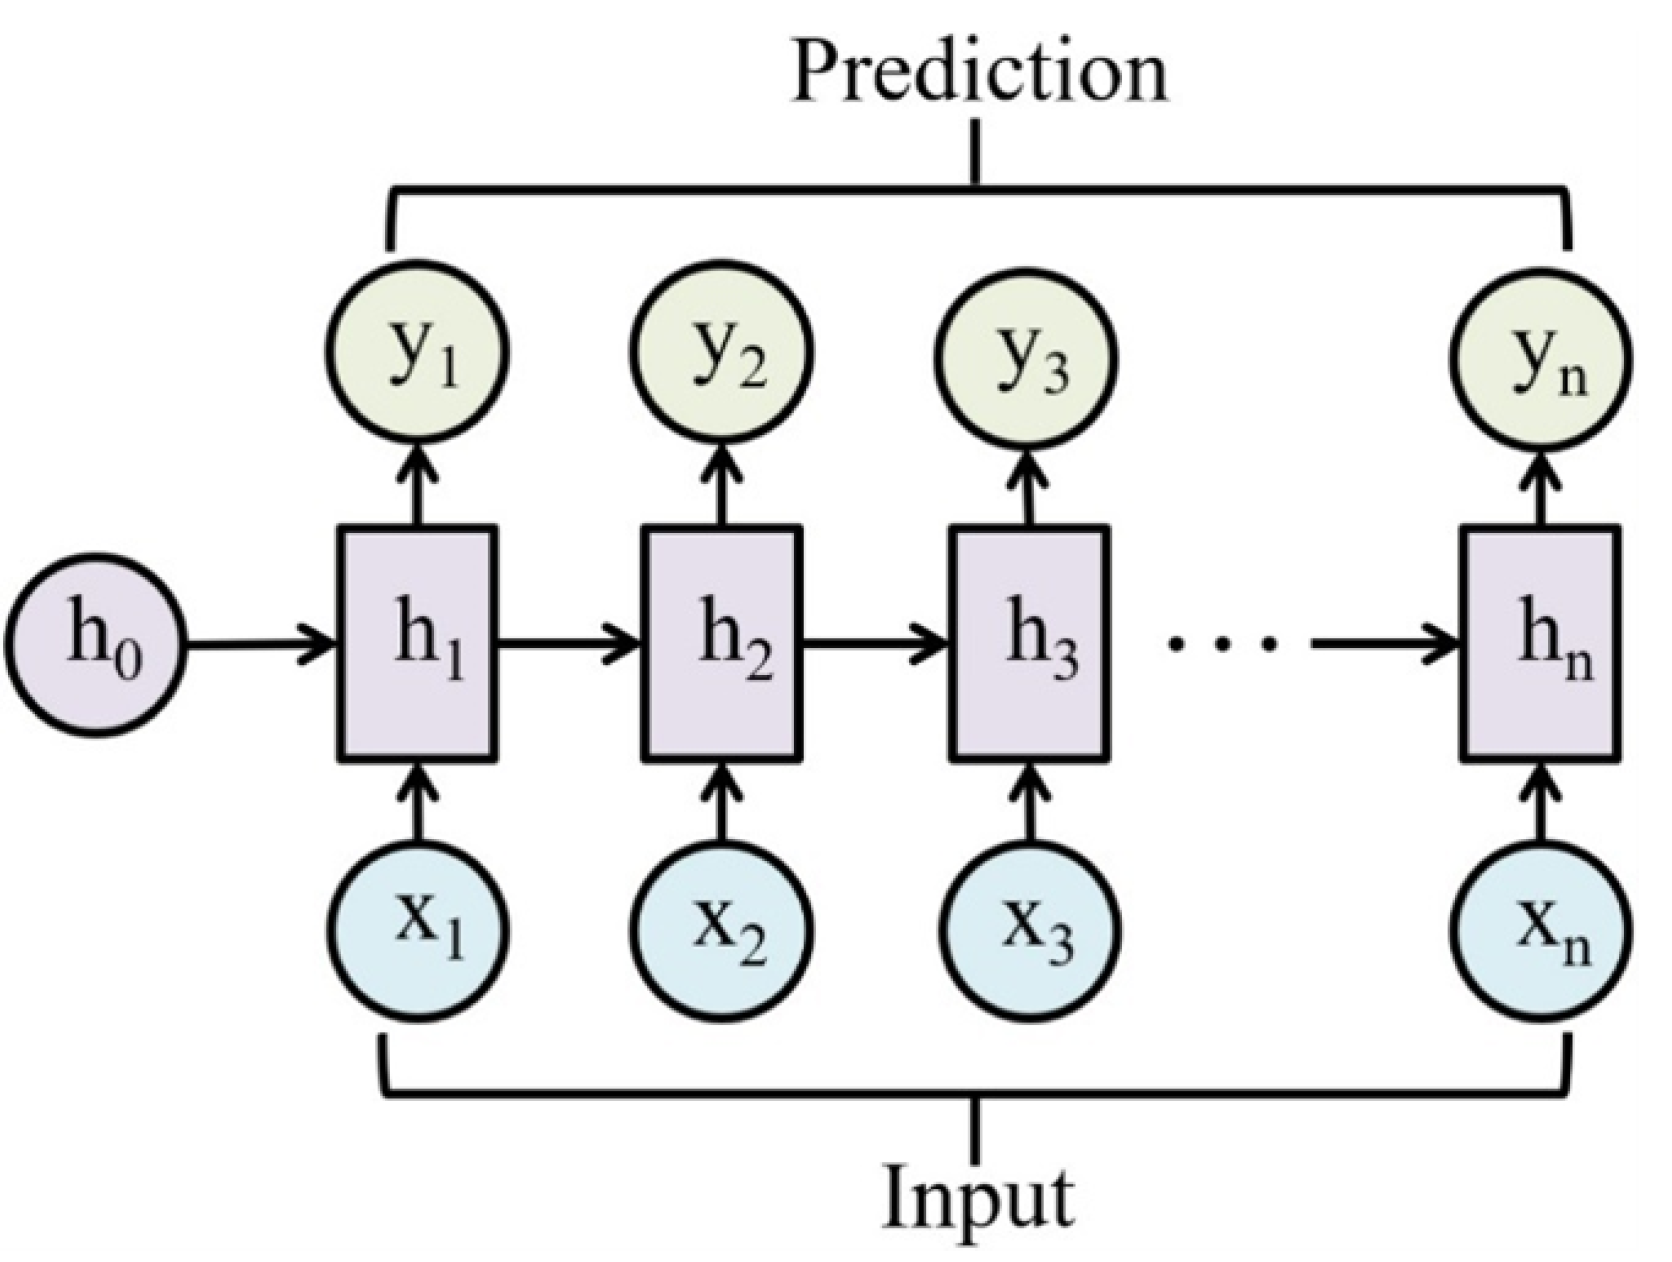
\includegraphics[width=0.5\textwidth]{rysunki/rnn.png}
            \captionof{figure}{ Schemat rekurencyjnej sieci neuronowej \cite{rnn_article2024}} 
            \label{rnn}
        \end{center}

        \noindent Istotnym wariantem rekurencyjnych sieci neuronowych, który sprawia, że  przestają one być \enquote{zapominalskie}, jest długa pamięć krótkotrwała (ang. \textit{long short-term memory} — LSTM). Sieci uczą się i zapamiętują długie sekwencje danych poprzez stan komórki (ang. \textit{cell state}) odzwierciedlający magistralę danych, której zawartość jest wybiórczo aktualizowana lub usuwana przez matematyczne mechanizmy bramek.

       Drugim kluczowym podejściem są konwolucyjne sieci neuronowe (ang. \textit{convolutional neural network} — CNN), które często wykorzystuje się w wizji komputerowej. Każde słowo w zdaniu może być zastąpione przez wektor słowa, a każdy z wektorów ma ten sam rozmiar. Taka struktura pomaga na ich pionowe zestawienie tworząc macierz o wymiarach $h \times w$, gdzie $h$ jest liczbą słów w zdaniu, a $w$ długością wektorów. Dane przygotowane w ten sposób przypominają strukturę obrazu, co umożliwia ich skuteczne przetwarzanie za pomocą CNN.